\documentclass[UTF8]{article}

%--
\usepackage{ctex}
\usepackage[margin=1in]{geometry}
\usepackage{graphicx}


%--
\begin{document}
    
%--
{\flushleft \bf \Large 姓名:} 杨佩成

{\flushleft \bf \Large 学号:} MG1733079

{\flushleft \bf \Large 日期:} 2017.11.20


%=========================================================================
\section*{论文信息}
    
Burrows M. The Chubby lock service for loosely-coupled distributed systems[C]// Symposium on Operating Systems Design and Implementation. USENIX Association, 2006:335-350.


    
\section{概述}
	Chubby是一个面向松耦合分布式系统的锁服务,其主要目标是要解决分布式系统中的一致性问题,例如分布式系统中leader的选取。此外,Chubby还提供了小数据量的存储服务,所以Chubby也被广泛用来提供命名服务和存储配置文件。Chubby的设计目标主要包括高可靠性、高可用性和易理解性,吞吐量和存储能力被放在次要位置。Chubby假设要解决的一致性问题是基于异步消息通信模型的,允许通信过程中存在丢包、延迟和重传,这一模型可以描述现实中的大多数网络。Chubby使用了Paxos算法来解决系统中的一致性问题。这篇论文主要是从工程性的角度出发,解释了Chubby中采用的方法和原因,并没有提出新的算法和内容。
%--
\section{设计}
	\subsection{基本原理}
	Chubby选择设计为锁服务而不是library主要是基于以下几点考虑:
\begin{itemize}
	\item
		开发人员在最初可能不会考虑系统的高可用性,但是随着系统的成熟和用户的增加,可用性越来越重		要,数据的复制和leader的选举就需要加入到设计中。锁服务可以方便的添加这些功能并且保持现有程序		的结构和通信模式。
	\item
		在广播服务结果时,需要Client读写一些小文件。这可以通过命名服务来实现,但是锁服务本身就可		以完成这个任务。
	\item
		程序员更加熟悉基于锁的接口。
	\item
		锁服务可以不需要基于Quorum做决定,这可以保证即使在客户系统的大多数成员没有启动时,客户系		统也可以做出正确的决定。
\end{itemize}

\indent 另外,Chubby中的锁是粗粒度的,粗粒度的锁可以持有几小时甚至几天。相比于细粒度的锁,粗粒度的锁对锁服务器的负载要少得多。但是粗粒度锁在不同客户端切换时会需要更多的操作,来保证服务器失效时能正常恢复。而细粒度的锁即使是短暂的失效也会导致许多客户端停止。Chubby中选择粗粒度锁提高了系统的可用性,放宽了一些性能上的要求。但是在Chubby中,用户也可以根据自己应用方便地实现自己的细粒度锁。
	\subsection{系统结构}

\begin{figure}[htbp]
\centering
\small
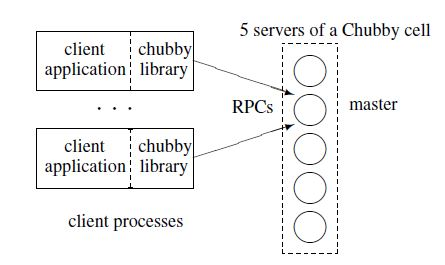
\includegraphics{1.JPG}
\caption{System structure}
\end{figure}
	Chubby主要由服务端和客户端两部分组成,二者通过RPC进行通信。每个客户端的应用都有一个Chubby library,客户端通过Chubby library与服务端交互,如Figure 1所示。
	
	每个Chubby cell都由一组服务器组成(一般是五台),每台服务器都作为一个副本,使用副本主要是为了防止单个节点的失效或者网络的异常,以达到高可靠性和高可用性的目标。同一个cell里的副本服务器维护的是同一个数据库的副本,只有master服务器可以处理数据库的读写请求,其他服务器只是通过一致性协议复制master里的更新。副本服务器通过分布式系统的一致性协议来选举master,master必须获得大多数副本服务器的投票并且在一个master租期中不会选出新的master。master的租期可以一直被延长,只要master能够一直赢得大多数服务器的选票。

	客户端通过向所有服务器发送master定位请求来找到master的位置,非master服务器收到请求会返回master的位置。当客户端知道了master的位置后,所有的请求就直接发送给master。写请求会通过一致性协议传播给其它服务器,当写操作在大多数服务器上完成后请求才会被答复。读请求只需要master就可以完成。

	当一台副本服务器宕机数小时后,系统会从后备机器中选择一台新的机器并在新的机器上启动锁服务,然后系统会在DNS列表中用新机器的ip替换掉故障机器的ip。master在检查DNS列表时会发现新的机器,然后就会更新cell数据库中的 副本成员。同时,新的副本服务器会从数据库中获取最新的备份,并根据其它活跃的服务器更新数据。当新的副本服务器处理了master等待确认的一条请求后,这台服务器才会在master选举中获得投票权。

\subsection{实现}
	Chubby本质上是一个分布式的、存储了大量小文件的文件系统,Chubby中的锁就是文件。用户通过操作文件,获取共享锁或独占锁。Chubby使用了一种类似于UNIX的文件系统,并做了一些针对分布式系统的优化:不提供文件的移动操作,不记录目录修改时间,不使用基于路径的权限管理。使用这种文件系统,简化了系统开发的工作量,并且也降低了Chubby用户的学习成本。在Chubby中文件和目录统称为node,每个node名在Chubby cell中都是唯一的。每个node都有很多元数据,包括存储了读、写、修改权限列表(ACL)的三个文件名以及文件版本号和校验和等元数据。Chubby通过类似于UNIX的Handle对node进行访问。Chubby中的每个node都可以作为一个读写锁,在写模式下客户端唯一的持有锁,在读模式下多个客户端可以共享锁。Chubby中实现的是Advisory lock而不是Mandatory lock,这么选择主要从以下几点考虑:Chubby锁通常是为了保护其它服务所使用的资源,若使用Mandatory lock会需要开发者对这些服务做更多的修改;使用Advisory lock能够访问加锁Node的数据,方便数据共享和调试。Chubby还为客户端提供事件订阅机制,包括了如下几种事件:文件内容修改,子节点改变和master故障等。引入事件通知,避免了客户端对服务器的轮询,也可以让客户端及时了解系统的变化。
	
	在分布式系统中锁是非常复杂的,因为通信的不确定和进程的失效,这会导致服务器处理的数据是乱序的。这种问题通常通过virtual time和virtual synchrony等算法解决。但是在现有的复杂系统上对所有的交互都引入序列号,代价是很高的,所以Chubby只对涉及到使用锁的交互操作引入序列号。锁的持有者可以请求一个sequencer,它包括了锁的名字、模式和锁的生成序号。当客户端需要执行被锁保护的操作时,客户端要将sequencer传给服务器。如果服务器判定sequencer无效,就会拒绝客户端的请求。
	尽管sequencer很容易使用,但是相关的重要协议发展得很慢。因此Chubby还提供了一种不完美但是能够在不支持sequencer场景下使用的算法。当客户端正常释放锁时,该锁可以被立即获取;但是如果因为客户端失效而锁被释放,锁服务器会在一段时间内拒绝其他客户端的锁请求。
	
	
	
	
	为了减少客户端与服务器之间的通信量,Chubby的客户端会缓存部分文件数据和节点的元数据。当缓存的数据要被修改时,修改的操作会被阻塞。同时master给缓存了这些数据的客户端发送失效信息,客户端收到失效信息后清空失效数据的缓存并回复。master在收到客户端回复的信息后才会真正执行修改操作,但是对读操作会立即响应,选择这种策略是因为Chubby中的读请求远大于写请求。另外,客户端还会缓存handle和lock。当lock被其他客户端请求时,服务器会以事件的形式通知缓存该lock的客户端释放lock。

	Chubby的服务器和客户端之间会维护一个会话,并通过周期性的握手(KeepAlive)来保证会话的有效性。只要会话是有效的,客户端的handle,lock和缓存数据就是有效的。客户端第一次连接到服务器时会请求一个会话,当客户端终止或者会话被闲置一段时间后,会话才会结束。每个会话都会有一个租期,master服务器可以自由延长会话的超时点。客户端会发送KeepAlive RPC,但是master并不会及时响应,它会在当前会话要结束时才会响应并通知客户端新的超时点。客户端在收到之前的KeepAlive响应后会立即发送新的KeepAlive,这样可以保证会话一直是有效的。KeepAlive还可以被用来传递事件信息和缓存失效信息。Chubby的客户端也会维护一个本地的租期超时点,这和服务器端的超时点不同,因为客户端认为通信是需要时间的。

	当客户端记录的本地超时点到达时,它会不确定是否是master终止了对话。客户端会进入jeopardy阶段,清空并禁用缓存。它会在这个状态等待一段时间,如果在这段时间里客户端能够重新与master建立连接,客户端就会恢复缓存的使用,否则就认为对话已结束。当刚进入jeopardy阶段时,客户端的Chubby library会通知应用进入静默状态,可以防止应用获取到不一致的数据。如果对话重新建立,应用就会继续运行而不必重新启动。这避免频繁对启动开销大的服务重复启动。

	当master发生故障或者失去了master身份时,它会丢弃掉内存中的状态包括会话、handle和锁等信息。服务器端的计时器会在新的master选举出来之前都停止,这可以延长会话在服务器端的租期。如果新的master很快被选出来,客户端可以在本地记录的会话超时之前与新的master重新建立连接。否则客户端就会进入jeopardy状态,等待一段时间,这样可以让会话在master发生失效时仍然维持下来。当客户端和新的master重新建立连接后,客户端的Chubby library要和master一起给应用提供未发生过失效的假象,这要求新的master恢复之前master内存里的信息。Chubby通过存储在外存上的数据、客户端的状态以及部分假设来恢复master内存的信息。
	
	每隔几个小时,每个Chubby cell的master都会把自己数据库的快照存储到另一个不同建筑里的GFS服务器中。将备份放在不同建筑中主要是为了让备份在房屋毁坏的情况下仍能恢复,同时也为了防止循环依赖(同一个建筑里的GFS可能会使用相同的Chubby cell选举master)。Chubby还允许将一组文件镜像到其它cell,这种镜像操作是很快的因为服务器中都是小文件并且事件通知机制可以及时通知文件的修改操作。
	
\section{总结}
	
	Chubby是一个给分布式系统提供粗粒度锁服务的系统,它还可以提供命名服务、存储配置信息。Chubby的设计思路主要基于以下几点:使用多个副本达到容错的目的并使用Paxos算法保证副本的一致性;使用客户端缓存和事件通知机制来减少服务器的负载;使用类似于文件系统的接口。
	
	Chubby虽然是一个为大量客户端提供服务的中心节点, 并没有花过多的精力在优化单条请求路径上,而是寻找可以减少master和客户端通信的机制,例如:客户端缓存几乎所有需要的信息;当负载较重时,master可以延长对话的租期。另外Chubby中还使用了责任分散的策略,将一些功能分散到不同的角色上。例如Chubby中发生写操作需要更新Client缓存时,master并没有去更新所有的客户端,而是让缓存失效,让客户端自己去更新缓存,这种推边拉的做法减少了master的压力,也降低了master设计的复杂度。Chubby中的这些设计策略对于我们设计其他系统很有指导意义。

	由于Chubby是要给其他系统提供锁服务,所以很多设计思路都是从使用锁服务的开放人员角度出发的。例如将整个系统设计为锁服务而不是library,避免需要开发人员大量修改原程序;使用类似于UNIX的文件系统,方便开发人员理解;使用advisory锁,方便调试和管理。作为google的基础系统,Chubby的设计方便了开发人员的使用。另外Chubby中的很大一部分设计都是为容错而设计,考虑到实际的应用环境,Chubby使用是异步通信模型,对于各种可能的错误都设计了解决方案,例如在Chubby cell中使用多台服务器作为副本,保证系统的可用性和可靠性;在客户端和服务器的会话中添加jeopardy状态,减少程序重启开销;定期对数据库备份并存储到不同位置的机器上,尽可能减少数据丢失的概率。这些设计的思路对于我们设计一些底层的分布式系统很有借鉴意义。



	


	





\end{document}

